\documentclass[main.tex]{subfiles}

\begin{document}
\section{Conclusioni}
In conclusione, i modelli migliori proposti nelle due analisi hanno la seguente capacità predittiva sull'insieme di test:\\
\begin{minipage}{0.45\textwidth}
\begin{figure}[H]
	\centering
	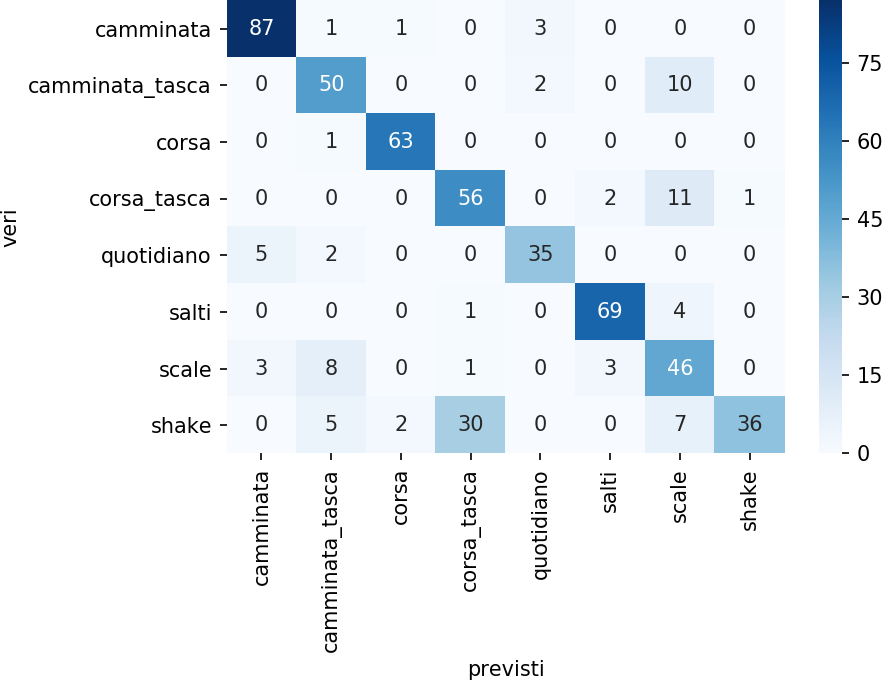
\includegraphics[width=\confusion]{../../figure/confusionMatrix-Mn-test.png}
	\caption{Matrice di confusione per il modello multinomiale nell'insieme di test, accuratezza dell'85.7\%.}
	\label{fig:mn-test}
\end{figure}
\end{minipage}
\hfill
\begin{minipage}{0.45\textwidth}
\begin{figure}[H]
	\centering
	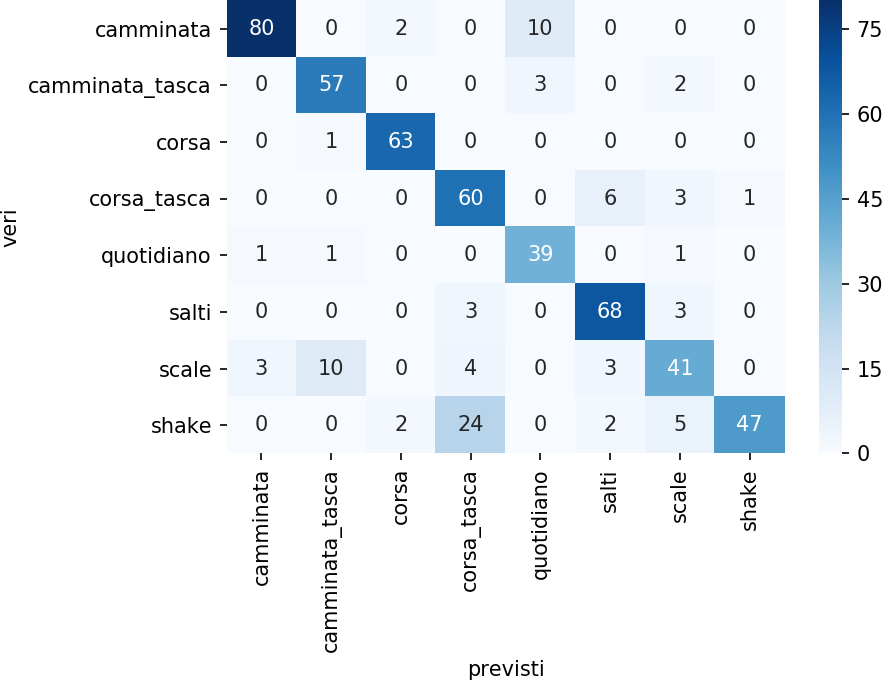
\includegraphics[width=\confusion]{../../figure/confusionMatrix-QDA-penalizzata-test.png}
	\caption{Matrice di confusione per la QDA pesata nell'insieme di test, accuratezza dell'83.5\%.}
	\label{fig:qda-test}
\end{figure}
\end{minipage}
\end{document}